\section{BGPmon: Using the Data}
\label{sec:usage}

\subsection{Receiving Routing Data}
BGPmon can provide a real-time routing event stream to a large number of clients. All routing events are integrated into two XML streams: update and RIB-IN streams. Both streams send ongoing messages in XML format. XML was chosen as the message format for the streams because it is extendable, for both clients and servers, and also readable by both applications and humans. 
%In our design, clients are able to subscribe to any XML stream. 

BGPmon peers with a number of routers (peers),  either directly or via chains to other BGPmon instances.   Each BGP update message\cite{bgprfc} from a peer is converted to XML format and forwarded to the update stream queue.    The resulting data can be filtered with simple parser libraries like LibXML2\cite{libxml2} or Expat\cite{expat}.  People, interested in receiving XML stream of BGP update events, should establish the TCP connection to BGPmon server \emph{livebgp.netsec.colostate.edu} port \emph{50001} or run simple telnet command to become familiar with XML message format.

BGPmon also stores RIB-IN tables on a per-peer basis. For each incoming BGP update message from a peer, BGPmon stores it in the peer's RIB-IN table. BGPmon periodically injects peer's route table into the XML RIB-IN stream. 
%Thereby, by receiving RIB-IN tables, clients are able to aggregate and analyze past events. 
XML RIB-IN event stream is available at \emph{livebgp.netsec.colostate.edu} port \emph{50002}. 

Also, BGPmon periodically announce XML \emph{status} messages to both the update and RIB-IN streams. \emph{Status} messages provide additional data about the load of BGPmon internal functions and summary information of each peer, for example, number of received BGP messages, prefixes, attributes and so on.

% produces additional XML messages to update and RIB-IN streams. These messages are \emph{status} messages. The main idea of these messages is to summarize routing information like number of prefix, attributes,  of BGPmon peers.

\subsection{An Example Use}


\begin{figure}
\centering
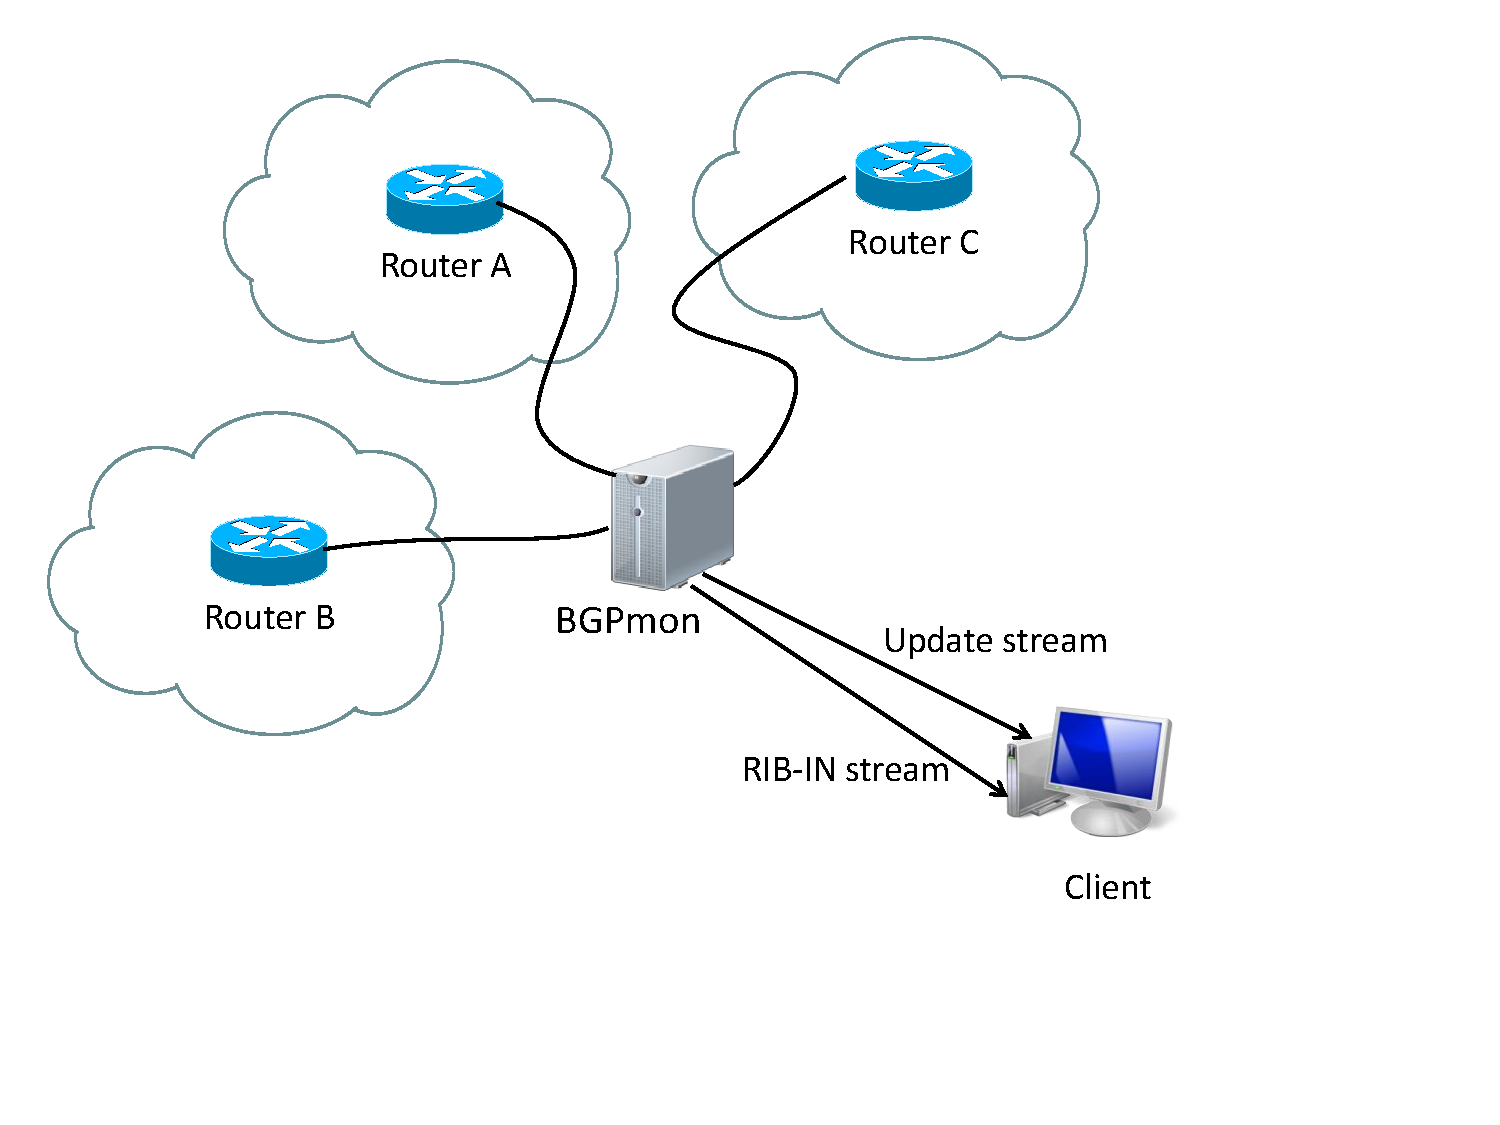
\includegraphics[scale=0.30]{figs/BGPmon-peers-with-client.pdf}
\caption{Receiving data from BGPmon}
\label{bgpmonclient}
\end{figure}

BGPmon clients are able to detect the possible BGP prefix hijack attacks.  For example,  suppose ISP A owns \emph{98.158.88/23}, \emph{98.158.90/23} and was assigned AS1000.  ISP A would like to monitor its prefixes and moreover, to receive an alert message when part or all network prefixes are announced by some misconfigured router with AS2000 number of ISP B (not shown in figure). To do it, ISP A should be a client of BGPmon and open two TCP connections to receive RIB-IN and update messages.

Figure\ref{bgpmonclient} shows a topology where BGPmon has BGP peering with three routers: Router A, B and C. Also, BGPmon has a client (ISP A).    To use the data, ISP A should establish connection to RIB-IN stream and receive a RIB-IN table snapshot. By filtering \emph{98.158.88/23} and \emph{98.158.90/23} prefixes and AS paths from snapshot, ISP A may see the \emph{current} routing picture how other routers (in our example, Routers A, B and C) in the Internet are able to reach ISP A subnets. In particular example, if Routers A,B and C can reach ISP A, their AS path should end with AS1000 number.

Next, ISP A should monitor the changes in AS path for its prefixes in real time. In order to do it, ISP A should establish a connection to update stream and constantly receive and filter XML messages. For instance, if some misconfigured router of ISP B will create a BGP announce message with \emph{98.158.88/23} prefix to Router B (see Figure\ref{bgpmonclient}), ISP A will be able to detect the problem easily by looking in AS path of Router B announce: the last AS number in AS path will be AS2000. Thus, by filtering real time XML data, ISP A is able to see \emph{precisely} when prefix \emph{98.158.88/23} was announced by malicious ISP B.  

This example shows the combination of the freely available BGPmon data streams can be combined with simple XML parsing to detect prefix hijacking as well as monitor the status of ISP routes.    The data can also be used a number of other ways and is limited only by the users ability to parse XML.
% Moreover, clients can filter XML data to monitor other important network attributes like AS path, source and destination IP addresses, AS numbers and so on.
% This simple example shows how clients are able to use routing event data to prevent and protect its router

%BGPmon provide a RIB-IN table stream every hour hours. 
%For every peer session, BGPmon    

%BGPmon stores RIB-IN tables on a per-peer basis. For each incoming BGP update message from a peer, BGPmon store it in the peer's RIB-IN table. BGPmon periodically injects peer's route table into the XML event stream. Thereby, by receiving RIB-IN tables, clients are able to aggregate and analyze past events. For instance, if client wants to see a list of prefixes historically originated or withdrew in past two hours, it should receive two table snapshots (by subscribing to RIB-IN stream), filter them and make simple diff operations. 









% Then, filter  with a simple XML parser routing events by its list of prefixes. To do is, ISP A has to For example, if prefix \emph{98.158.90/23} is announced by another ISP B, ISP A will detect the exact moment when BGP update was generated. Moreover, ISP A is able to monitor an AS path in update stream

%can easily subscribe to an update XML stream and receive a live XML data, which could be analyzed, filtered against corruption of Internet routing tables. 

% RouteViews system only allows hijack alert systems to report hijacks that occurred many minutes ago.




% For example, BGPmon update stream is able to predict possible BGP prefix hijacking attacks. Clients, interested in monitoring its own list of prefixes appeared in other peer announcements, can easily subscribe to an update XML stream and receive a live XML data, which could be analyzed, filtered against corruption of Internet routing tables. Moreover, BGPmon provide a RIB-IN table stream every hour hours. For instance, if clients want to see a list of prefixes historically originated or withdrew in past two hours, they should receive two table snapshots (by subscribing to RIB-IN stream) and make simple diff operations. 




%For example, if client wants to monitor its own list of prefixes (to prevent possible BGP hijack attacks) appeared in other peer announcements, it should subscribe to an update XML stream. By monitoring update stream, client could prevent a possible BGP hijack attacks. 

%Also, to receive a full RIB-IN table every two hours, client should connect to BGPmon RIB-IN XML stream.  



%For example, using BGPmon update stream, client can prevent a possible BGP hijack prefix attacks. To do it, client should develop a simple XML parser, which will receive routing events from BGPmon. 



%People, interested in receiving a XML stream of routing events from BGPmon, should open a TCP connection (or simply run telnet) to BGPmon main server \emph{lisa.netsec.colostate.edu} (129.82.138.26) port \emph{50001}. XML RIB-IN event stream is available at \emph{lisa.netsec.colostate.edu} (129.82.138.26) port \emph{50002}.

%BGPMon 7.2 has been running stable for two years at Network Security Lab, Colorado State University which has a BGP peering with 7 ISPs and peering with 3 Oregon RouteViews\cite{routeviews} collectors (more than 80 peers around the world).

%\subsection{BGPmon deployment}